\chapter{Luyện tập: Từ trường của dòng điện chạy trong các dây dẫn có hình dạng đặc biệt}
\section{Chạy trong dây dẫn thẳng dài}
\begin{enumerate}
	\item {Dòng điện chạy qua một dây dẫn thẳng dài đặt nằm ngang trong không khí gây ra tại một điểm cách nó 4,5 cm một cảm ứng từ có độ lớn $\text{2,8}\cdot 10^{-4}\ \text{T}$. Cường độ của dòng điện chạy qua dây dẫn là 
		\begin{mcq}(4)
			\item 56 A.			
			\item 44 A.				
			\item 63 A.				
			\item 8,6 A.
		\end{mcq}
	}
	\item {Dòng điện chạy qua một dây dẫn thẳng dài đặt nằm ngang trong không khí gây ra tại một điểm cách nó 4,5 cm một cảm ứng từ có độ lớn $\text{2,8}\cdot 10^{-5}\ \text{T}$. Độ lớn của cảm ứng từ do dòng điện này gây ra tại điểm cách nó 10 cm là
		\begin{mcq} (4)
			\item $\text{1,26}\cdot 10^{-5}\ \text{T}$.		
			\item $\text{1,24}\cdot 10^{-5}\ \text{T}$.			
			\item $\text{1,38}\cdot 10^{-5}\ \text{T}$.			
			\item $\text{8,6}\cdot 10^{-5}\ \text{T}$.	
		\end{mcq}	
	}
	\item {Dòng điện thẳng dài I và hai điểm M, N nằm trong cùng mặt phẳng, nằm cùng phía so với dòng điện sao cho MN vuông góc với dòng điện. Gọi O là trung điểm của MN. Nếu độ lớn cảm ứng từ tại M và N lần lượt là $\text{BM}=\text{2,8}\cdot 10^{-5}\ \text{T}$, $\text{BN}=\text{4,2}\cdot 10^{-5}\ \text{T}$ thì độ lớn cảm ứng từ tại O là?
		\begin{mcq} (4)
			\item $\text{3,36}\cdot 10^{-5}\ \text{T}$.		
			\item $\text{16,8}\cdot 10^{-5}\ \text{T}$.			
			\item $\text{3,5}\cdot 10^{-5}\ \text{T}$.			
			\item $\text{56}\cdot 10^{-5}\ \text{T}$.	
		\end{mcq}	
	}
\end{enumerate}

\textbf{ĐÁP ÁN}
\begin{longtable}[\textwidth]{|p{0.1\textwidth}|p{0.1\textwidth}|p{0.1\textwidth}|p{0.1\textwidth}|p{0.1\textwidth}|p{0.1\textwidth}|p{0.1\textwidth}|p{0.1\textwidth}|}
	% --- first head
	\hline%\hspace{2 pt}
	\multicolumn{1}{|c}{\textbf{Câu 1}} & \multicolumn{1}{|c|}{\textbf{Câu 2}} & \multicolumn{1}{c|}{\textbf{Câu 3}} &
	\multicolumn{1}{c|}{\textbf{Câu 4}} &
	\multicolumn{1}{c|}{\textbf{Câu 5}} &
	\multicolumn{1}{c|}{\textbf{Câu 6}} &
	\multicolumn{1}{c|}{\textbf{Câu 7}} &
	\multicolumn{1}{c|}{\textbf{Câu 8}} \\
	\hline
	C.&A. &A. & & & & &\\
	\hline
\end{longtable}

\section{Chạy trong dây dẫn uốn thành vòng tròn và khung dây}
\begin{enumerate}
	\item {Khi cho dòng điện cường độ 10 A chạy qua một vòng dây dẫn đặt trong không khí thì cảm ứng từ tại tâm của vòng dây dẫn có độ lớn là $\text{2,1}\cdot 10^{-4}\ \text{T}$. Xác định bán kính của vòng dây.
		\begin{mcq}(4)
			\item 5,0 cm.			
			\item 0,30 cm.			
			\item 3,0 cm.		
			\item 2,5 cm.
		\end{mcq}
	}
	\item {Một vòng dây tròn đặt trong chân không có bán kính R mang dòng điện có cường độ $I$ thì cảm ứng từ tại tâm vòng dây là $10\ \mu \text{T}$. Nếu cho dòng điện trên qua vòng dây có bán kính $4R$ thì cảm ứng từ tại tâm vòng dây có độ lớn là
		\begin{mcq} (4)
			\item $6 \cdot 10^{-6}\ \text{T}$.			
			\item $\text{1,2}\cdot 10^{-6}\ \text{T}.$			
			\item $15 \cdot 10^{-6}\ \text{T}$.		
			\item $\text{2,5}\cdot 10^{-6}\ \text{T}.$	
		\end{mcq}
	}
	\item{Khung dây tròn đặt trong không khí bán kính 30 cm có 100 vòng dây. Cường độ dòng điện qua khung dây là $\dfrac{\text{0,3}}{\pi}\ \text{A}$. Độ lớn cảm ứng từ tại tâm khung dây là 
		\begin{mcq}(4)
			\item $4 \cdot 10^{-5}\ \text{T}$.		
			\item $2 \cdot 10^{-5}\ \text{T}$.			
			\item $\text{6,28}\cdot 10^{-5}\ \text{T}.$	 		
			\item $\text{9,42}\cdot 10^{-5}\ \text{T}.$	
		\end{mcq}
	}
	\item {Dùng một dây đồng có phủ một lớp sơn cách điện mỏng, quấn quanh một hình trụ dài $L = 50\ \text{cm}$, có đường kính $d = 4\ \text{cm}$ để làm một ống dây. Sợi dây quấn Ống dây có chiều dài $l = 314\ \text{cm}$ và các vòng dây được quấn sát nhau. Hỏi nếu cho dòng điện cường độ $I = \text{0,4}\ \text{A}$ chạy qua ống dây, thì cảm ứng từ bên trong ống dây bằng bao nhiêu?
		\begin{mcq}(4)
			\item $5 \cdot 10^{-5}\ \text{T}$.			
			\item $\text{2,5}\cdot 10^{-5}\ \text{T}.$				
			\item $\text{1,25}\cdot 10^{-5}\ \text{T}.$				
			\item $3 \cdot 10^{-5}\ \text{T}$.	
		\end{mcq}
	}
	\item {Một vòng dây tròn đặt trong chân không có bán kính $R = 10\ \text{cm}$ mang dòng điện $I = 50\ \text{A}$. Tính độ lớn của vecto cảm ứng từ tại tâm vòng dây.
		\begin{mcq}(4)
			\item $\text{31,4}\cdot 10^{-5}\ \text{T}.$		
			\item $10\cdot 10^{-5}\ \text{T}.$		
			\item $20\cdot 10^{-5}\ \text{T}.$		
			\item $\text{3,14}\cdot 10^{-5}\ \text{T}.$	
		\end{mcq}
	}
	\item {Một vòng dây tròn đặt trong chân không có bán kính $R = 10\ \text{cm}$ mang dòng điện $I = 50\ \text{A}$. Nếu cho dòng điện trên qua vòng dây có bán kính $R = 4R$ thì cảm ứng từ tại tâm vòng dây có độ lớn là bao nhiêu?
		\begin{mcq}(4)
			\item $\text{31,4}\cdot 10^{-5}\ \text{T}.$	 	
			\item $\text{15,7}\cdot 10^{-5}\ \text{T}.$	
			\item $\text{7,85}\cdot 10^{-5}\ \text{T}.$		
			\item $\text{10,46}\cdot 10^{-5}\ \text{T}.$	
		\end{mcq}
	}
\end{enumerate}

\textbf{ĐÁP ÁN}
\begin{longtable}[\textwidth]{|p{0.1\textwidth}|p{0.1\textwidth}|p{0.1\textwidth}|p{0.1\textwidth}|p{0.1\textwidth}|p{0.1\textwidth}|p{0.1\textwidth}|p{0.1\textwidth}|}
	% --- first head
	\hline%\hspace{2 pt}
	\multicolumn{1}{|c}{\textbf{Câu 1}} & \multicolumn{1}{|c|}{\textbf{Câu 2}} & \multicolumn{1}{c|}{\textbf{Câu 3}} &
	\multicolumn{1}{c|}{\textbf{Câu 4}} &
	\multicolumn{1}{c|}{\textbf{Câu 5}} &
	\multicolumn{1}{c|}{\textbf{Câu 6}} &
	\multicolumn{1}{c|}{\textbf{Câu 7}} &
	\multicolumn{1}{c|}{\textbf{Câu 8}} \\
	\hline
	C.&D. &B. &B. &A. &C. & &\\
	\hline
	
\end{longtable}

\section{Từ trường của nhiều dòng điện}
\begin{enumerate}
	\item {Một dây dẫn thẳng, dài có vỏ bọc cách điện, ở khoảng giữa được uốn thành vòng tròn, bán kính $R = 20\ \text{cm}$ như hình vẽ. Dòng điện chạy qua dây dẫn có cường độ 5 A. Xác định cảm ứng từ tại tâm O của vòng tròn.
		\begin{mcq}(4)
			\item $5 \cdot 10^{-6}\ \text{T}$.			
			\item $\text{15,7}\cdot 10^{-6}\ \text{T}.$		
			\item $\text{10,7}\cdot 10^{-6}\ \text{T}.$		
			\item $\text{20,7}\cdot 10^{-6}\ \text{T}.$	
		\end{mcq}
	}
	\item{Một dây dẫn rất dài được căng thẳng trừ một đoạn ở giữa dây uốn thành một vòng tròn bán kính 1,5 cm. Cho dòng điện 3 A chạy trong dây dẫn. Xác định cảm ứng từ tại tâm của vòng tròn nếu vòng tròn và phần dây thẳng cùng nằm trong một mặt phẳng:	 
		\begin{center}
			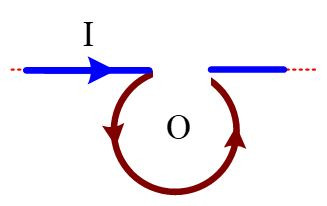
\includegraphics[scale=0.6]{../figs/VN11-PH-26-P-017-1-1.JPG}
		\end{center}
		\begin{mcq}(4)
			\item $\text{5,6}\cdot 10^{-5}\ \text{T}.$				
			\item $\text{6,6}\cdot 10^{-5}\ \text{T}.$			
			\item $\text{7,6}\cdot 10^{-5}\ \text{T}.$		
			\item $\text{8,6}\cdot 10^{-5}\ \text{T}.$	
		\end{mcq}
		
	}
	\item{Một dây dẫn rất dài được căng thẳng trừ một đoạn ở giữa dây uốn thành một vòng tròn bán kính 1,5 cm. Cho dòng điện 3 A chạy trong dây dẫn. Xác định cảm ứng tù tại tâm của vòng tròn nếu vòng tròn và phần dây thẳng cùng nằm trong một mặt phẳng, chỗ bắt chéo hai đoạn dây không nối với nhau:
		\begin{center}
			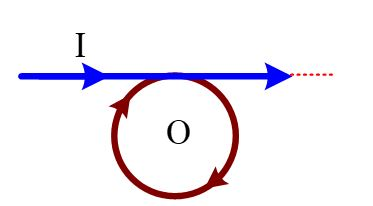
\includegraphics[scale=0.6]{../figs/VN11-PH-26-P-017-1-2.JPG}
		\end{center}	 
		
		\begin{mcq}(4)
			\item $\text{15,6}\cdot 10^{-5}\ \text{T}.$				
			\item $\text{16,6}\cdot 10^{-5}\ \text{T}.$			
			\item $\text{17,6}\cdot 10^{-5}\ \text{T}.$		
			\item $\text{18,6}\cdot 10^{-5}\ \text{T}.$	
		\end{mcq}
		
	}
	\item {Hai dòng điện đặt trong không khí đồng phẳng: dòng thứ nhất thẳng đều, có cường độ $I_1 = 2\ \text{A}$, dòng thứ hai hình tròn, tâm $\text{O}_2$ cách dòng thứ nhất 40 cm, bán kính $R_2 = 20\ \text{cm}$, có cường độ $I_2 = \dfrac{4}{\pi}\ \text{A}$. Xác định độ lớn cảm ứng từ tại tâm $\text{O}_2$
		\begin{center}
			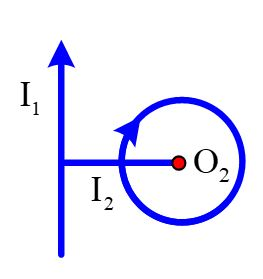
\includegraphics[scale=0.6]{../figs/VN11-PH-26-P-017-1-3.JPG}
		\end{center}	
		\begin{mcq}(4)
			\item $6 \cdot 10^{-6}\ \text{T}$.			
			\item $4 \cdot 10^{-6}\ \text{T}.$		
			\item $5 \cdot 10^{-6}\ \text{T}.$		
			\item $3 \cdot 10^{-6}\ \text{T}.$	
		\end{mcq}
		
	}
	\item{Hai vòng tròn dây dẫn đồng tâm, bán kính vòng thứ nhất là $R = 8\ \text{cm}$, vòng thứ 2 là $2R$ trong mỗi vòng có dòng điện cường đội $I = 10\ \text{A}$ chạy qua. Nếu hai vòng dây nằm trong cùng một mặt phẳng và $I$ cùng chiều thì đọ lớn cảm ứng từ tống hợp tại O là:
		\begin{mcq}(4)
			\item $\text{11,78}\cdot 10^{-5}\ \text{T}.$				
			\item $\text{2,12}\cdot 10^{-5}\ \text{T}.$			
			\item $\text{0,71}\cdot 10^{-5}\ \text{T}.$		
			\item $\text{3,93}\cdot 10^{-5}\ \text{T}.$	
		\end{mcq}
		
		
	}
	\item{Hai dây dẫn thẳng song song dài vô hạn đặt cách nhau 10 cm trong không khí. Dòng điện chạy trong 2 dây dẫn ngược chiều nhau và có cường độ $I_1 = 10\ \text{A}$; $I_2 = 20\ \text{A}$. Tìm cảm ứng từ tại:
		a) Điểm A cách mỗi dây 5 cm.
		\begin{mcq}(4)
			\item $4 \cdot 10^{-5}\ \text{T}$.			
			\item $8 \cdot 10^{-5}\ \text{T}.$		
			\item $12 \cdot 10^{-5}\ \text{T}.$		
			\item $16 \cdot 10^{-5}\ \text{T}.$	
		\end{mcq}	
		b) Điểm B cách dây 1 đoạn 4 cm cách dây 2 đoạn 14 cm
		\begin{mcq}(4)
			\item $\text{7,857}\cdot 10^{-5}\ \text{T}.$				
			\item $\text{2,143}\cdot 10^{-5}\ \text{T}.$			
			\item $\text{4,286}\cdot 10^{-5}\ \text{T}.$		
			\item $\text{3,929}\cdot 10^{-5}\ \text{T}.$	
		\end{mcq}
		
		c) Điểm M cách mỗi dây 10 cm.
		\begin{mcq}(4)
			\item $2\cdot 10^{-5}\ \text{T}.$				
			\item $4\cdot 10^{-5}\ \text{T}.$			
			\item $\text{3,464}\cdot 10^{-5}\ \text{T}.$		
			\item $\text{4,472}\cdot 10^{-5}\ \text{T}.$	
		\end{mcq}
		
		d) Điểm N cách dây 1 đoạn 8 cm và cách dây 2 đoạn 6 cm
		\begin{mcq}(4)
			\item $\text{2,5}\cdot 10^{-5}\ \text{T}.$				
			\item $\text{6,67}\cdot 10^{-5}\ \text{T}.$			
			\item $\text{7,12}\cdot 10^{-5}\ \text{T}.$		
			\item $\text{6,18}\cdot 10^{-5}\ \text{T}.$	
		\end{mcq}
		
	}
	\item {Hai dây dẫn thẳng, rất dài, đặt trong không khí, trùng với hai trục tọa độ vuông góc $\text{xOy}$. Dòng điện qua dây $\text{Ox}$ chạy cùng chiều với chiều dương của trục tọa độ và có cường độ bằng 2 A, dòng điện qua dây $\text{Oy}$ chạy ngược chiều với chiều dương của trục tọa độ và có cường độ $\dfrac{2}{3}\ \text{A}$. Xác đinh cảm ứng từ tổng hợp do hai dòng điện này gây ra tại điểm A có tọa độ $x = 4\ \text{cm}$ và $y = -2\ \text{cm}$.
		\begin{mcq}(4)
			\item $\text{0,5}\cdot 10^{-5}\ \text{T}.$				
			\item $2\cdot 10^{-5}\ \text{T}.$			
			\item $\text{1,5}\cdot 10^{-5}\ \text{T}.$		
			\item $\text{3,5}\cdot 10^{-5}\ \text{T}.$	
		\end{mcq}
	}
	\item {Ba dòng điện thẳng song song vuông góc với mặt phẳng hình vẽ. Khoảng cách từ điểm M đến ba dòng điện trên mô tả như hình vẽ. Xác định véc tơ cảm ứng từ tại M trong trường hợp cả ba dòng điện đều 
		\begin{center}
			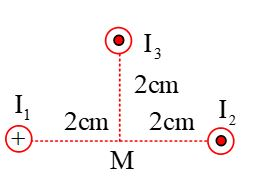
\includegraphics[scale=0.6]{../figs/VN11-PH-26-P-017-1-4.JPG}
		\end{center}
		\begin{mcq}(4)
			\item $10^{-4}\ \text{T}.$				
			\item $2\cdot 10^{-4}\ \text{T}.$			
			\item $3\cdot 10^{-4}\ \text{T}.$		
			\item $4\cdot 10^{-4}\ \text{T}.$
		\end{mcq}
	}
	\item {Ba dòng điện thẳng song song vuông góc với mặt phẳng hình vẽ, có chiều như hình vẽ. ABCD là hình vuông cạnh 10 cm, $I_1 = I_2 = I_3 = 5\ \text{A}$, xác định véc tơ cảm ứng từ tại đỉnh thứ tư D của hình vuông:
		\begin{center}
			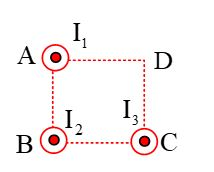
\includegraphics[scale=0.6]{../figs/VN11-PH-26-P-017-1-5.JPG}
		\end{center}
		\begin{mcq}(4)
			\item $\text{1,2}\sqrt 3 \cdot 10^{-5}\ \text{T}.$			\item $1\sqrt 3 \cdot 10^{-5}\ \text{T}.$			
			\item $\text{1,5}\sqrt 2 \cdot 10^{-5}\ \text{T}.$		
			\item $\text{2,4}\sqrt 2 \cdot 10^{-5}\ \text{T}.$
		\end{mcq}
	}
	\item {Hai dây dẫn thẳng, rất dài, đặt song song, cách nhau 20 cm trong không khí, có hai dòng điện ngược chiều, có cường độ $I_1 = 12\ \text{A}$; $I_2 = 15\ \text{A}$ chạy qua. Xác định cảm ứng từ tổng hợp do hai dòng điện này gây ra tại điểm M cách dây dẫn mang dòng $I_1$ một đoạn 15 cm và cách dây dẫn mang dòng $I_2$ một đoạn 5 cm.
		\begin{mcq}(4)
			\item $\text{1,6}\cdot 10^{-5}\ \text{T}.$				
			\item $6\cdot 10^{-5}\ \text{T}.$			
			\item $\text{7,6}\cdot 10^{-5}\ \text{T}.$		
			\item $\text{4,4}\cdot 10^{-5}\ \text{T}.$	
		\end{mcq}
	}
	\item{Hai dây dẫn thẳng dài song song cách nhau một khoảng cố định 42 cm. Dây thứ nhất mang dòng điện 3 A, dây thứ hai mang dòng điện 1,5 A, nếu hai dòng điện ngược chiều, những điểm mà tại đó cảm ứng từ bằng không nằm trên đường thẳng:
		\begin{mcq}
			\item song song với $I_1$, $I_2$ và cách $I_1$ 28 cm.
			\item nằm giữa hai dây dẫn, trong mặt phẳng và song song với $I_1$, $I_2$ và cách $I_2$ 14 cm.
			\item trong mặt phẳng và song song với $I_1$, $I_2$ nằm ngoài khoảng giữa hai dòng điện gần $I_2$ cách $I_2$ 42 cm.
			\item song song với $I_1$, $I_2$ và cách $I_2$ 20 cm. 
		\end{mcq}
	}
\end{enumerate}

\textbf{ĐÁP ÁN}
\begin{longtable}[\textwidth]{|m{0.1\textwidth}|m{0.1\textwidth}|m{0.1\textwidth}|m{0.1\textwidth}|m{0.1\textwidth}|m{0.1\textwidth}|m{0.1\textwidth}|m{0.1\textwidth}|}
	% --- first head
	\hline%\hspace{2 pt}
	\multicolumn{1}{|c}{\textbf{Câu 1}} & \multicolumn{1}{|c|}{\textbf{Câu 2}} & \multicolumn{1}{c|}{\textbf{Câu 3}} &
	\multicolumn{1}{c|}{\textbf{Câu 4}} &
	\multicolumn{1}{c|}{\textbf{Câu 5}} &
	\multicolumn{1}{c|}{\textbf{Câu 6}} &
	\multicolumn{1}{c|}{\textbf{Câu 7}} &
	\multicolumn{1}{c|}{\textbf{Câu 8}}  \\
	\hline
	C.&D. &B. &D. &A. &\begin{enumerate}[label=\alph*)]
		\item C.
		\item B.
		\item C.
		\item C.
	\end{enumerate}&A. &A.\\
	\hline
	
	\multicolumn{1}{|c|}{\textbf{Câu 9}} & \multicolumn{1}{c|}{\textbf{Câu 10}} & \multicolumn{1}{c|}{\textbf{Câu 11}} &
	\multicolumn{1}{c|}{\textbf{Câu 12}} &
	\multicolumn{1}{c|}{\textbf{Câu 13}} &
	\multicolumn{1}{c|}{\textbf{Câu 14}} &
	\multicolumn{1}{c|}{\textbf{Câu 15}} &
	\multicolumn{1}{c|}{\textbf{Câu 16}} \\
	\hline
	C. &C. &C. & && & &	\\
	\hline
\end{longtable}


